
\documentclass[paper=a4, fontsize=11pt]{scrartcl} % A4 paper and 11pt font size
\usepackage[T1]{fontenc} % Use 8-bit encoding that has 256 glyphs
\usepackage[english]{babel} 
\usepackage{amsmath,amsfonts,amsthm} 
\usepackage{graphicx}
\usepackage{caption}
\usepackage{subcaption}
\numberwithin{figure}{section} 
\setlength\parindent{0pt} % Removes all indentation from paragraphs - comment this line for an assignment with lots of text


\title{	
\normalfont \normalsize 
\textsc{Practical exercise with ARTS, OSF SoSe15} \\ [25pt] % Your university, school and/or department name(s)
%\horrule{0.5pt} \\[0.4cm] % Thin top horizontal rule
\huge Exercise 1: Calculation of Absorption Coefficients  \\ % The assignment title
}

\author{sample solution}
\date{\normalsize\today} 

\begin{document}

\maketitle

\section{absorption cross sections of different molecules}

Calculate the absorption cross sections in the microwave spectral range for the following molecules: 
\begin{itemize}
	\item HCl
	\item ClO
	\item CO
	\item $N_{2}O$
	\item $O_{3}$
\end{itemize}
(Unless otherwise specified use the parameter setting as given in the example file 'absorption.arts'.)	

% figures abs cross sections
\begin{figure}[t!]
 \centering
 \begin{subfigure}[t]{0.45\textwidth}
 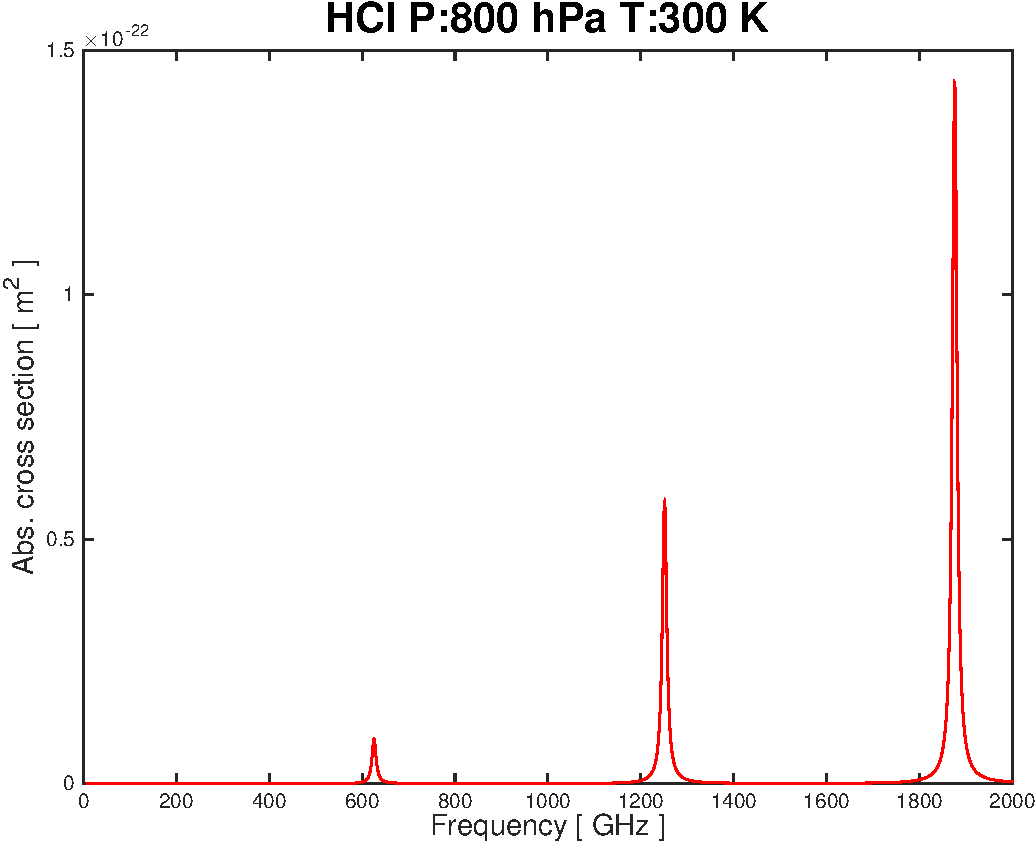
\includegraphics[width=\textwidth]{plots/plot_xsec_HCl_800hPa_300K.pdf}
 \caption{HCl}
 \end{subfigure}
 \begin{subfigure}[t]{0.45\textwidth}
 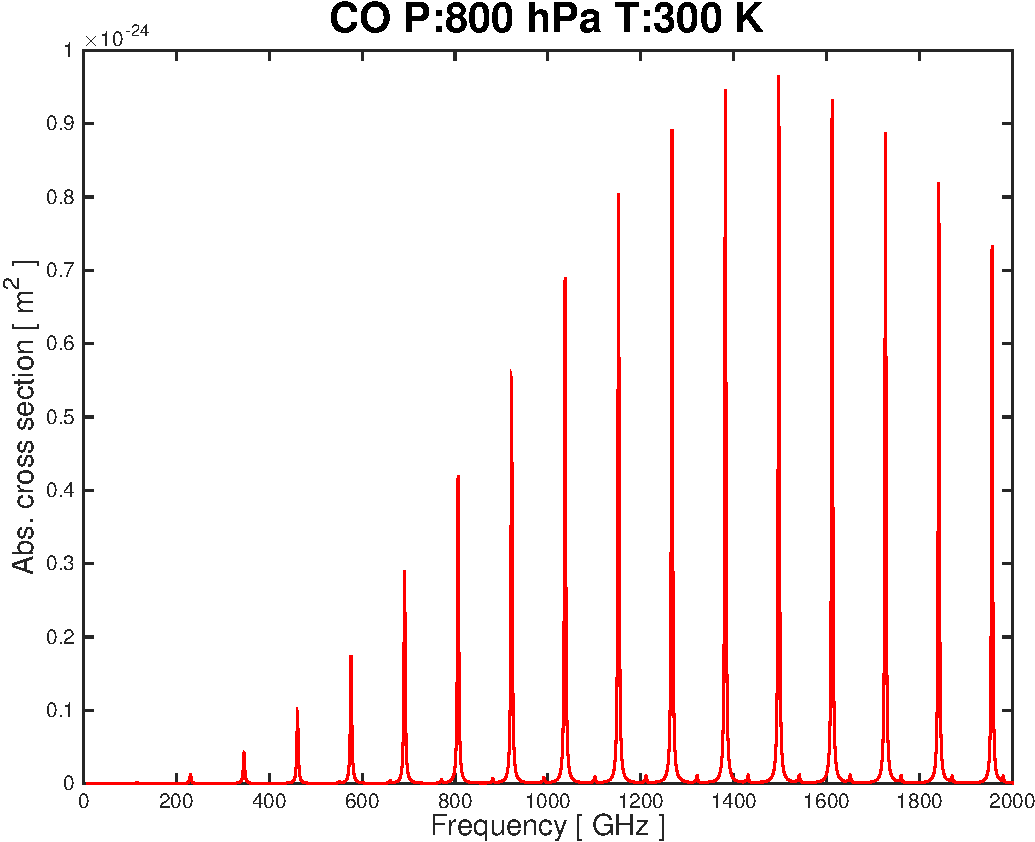
\includegraphics[width=\textwidth]{plots/plot_xsec_CO_800hPa_300K.pdf}
 \caption{CO}
 \end{subfigure}
 
 \begin{subfigure}[b]{0.45\textwidth}
 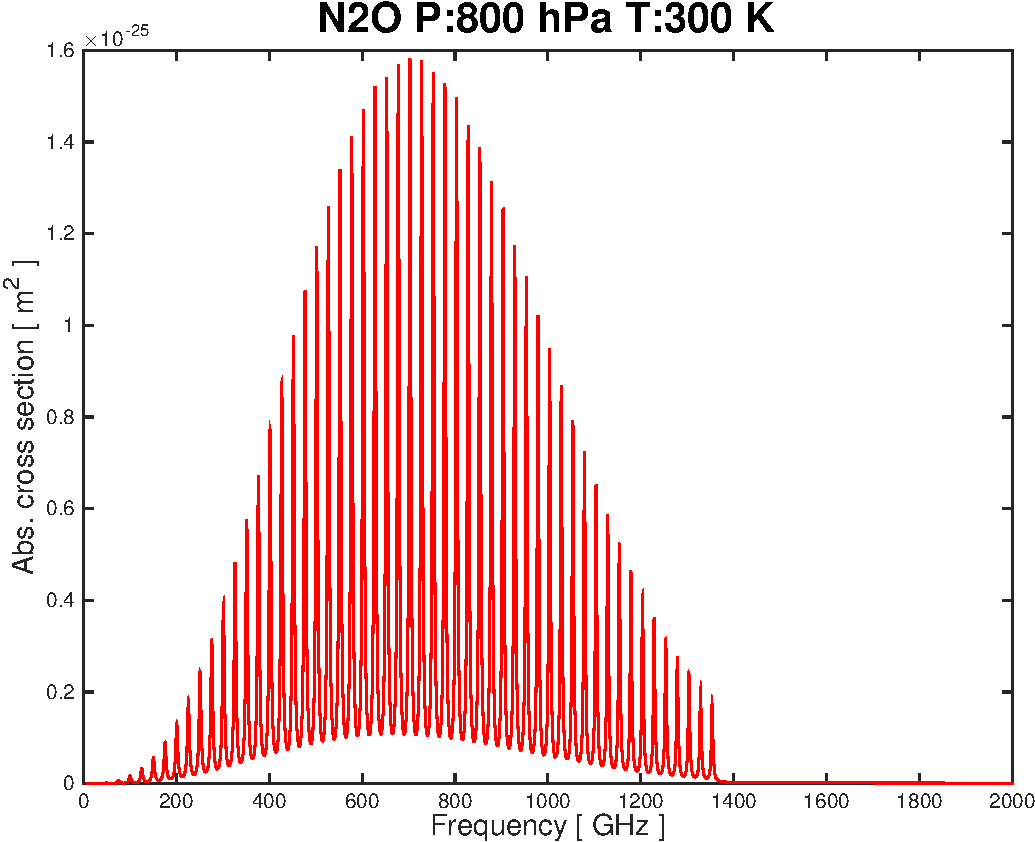
\includegraphics[width=\textwidth]{plots/plot_xsec_N2O_800hPa_300K.pdf}
 \caption{N2O}
 \end{subfigure}  
 \begin{subfigure}[b]{0.45\textwidth}
 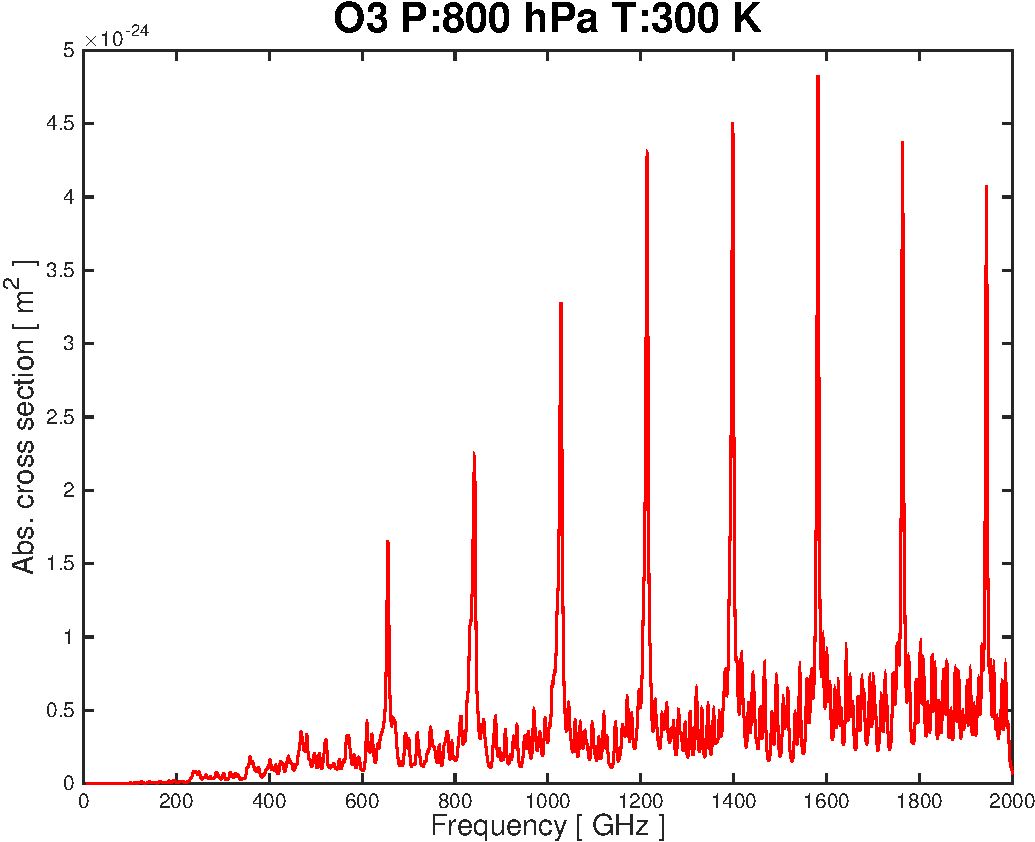
\includegraphics[width=\textwidth]{plots/plot_xsec_O3_800hPa_300K.pdf}
 \caption{O3}
 \end{subfigure}
 
 \begin{subfigure}[b]{0.45\textwidth} 
 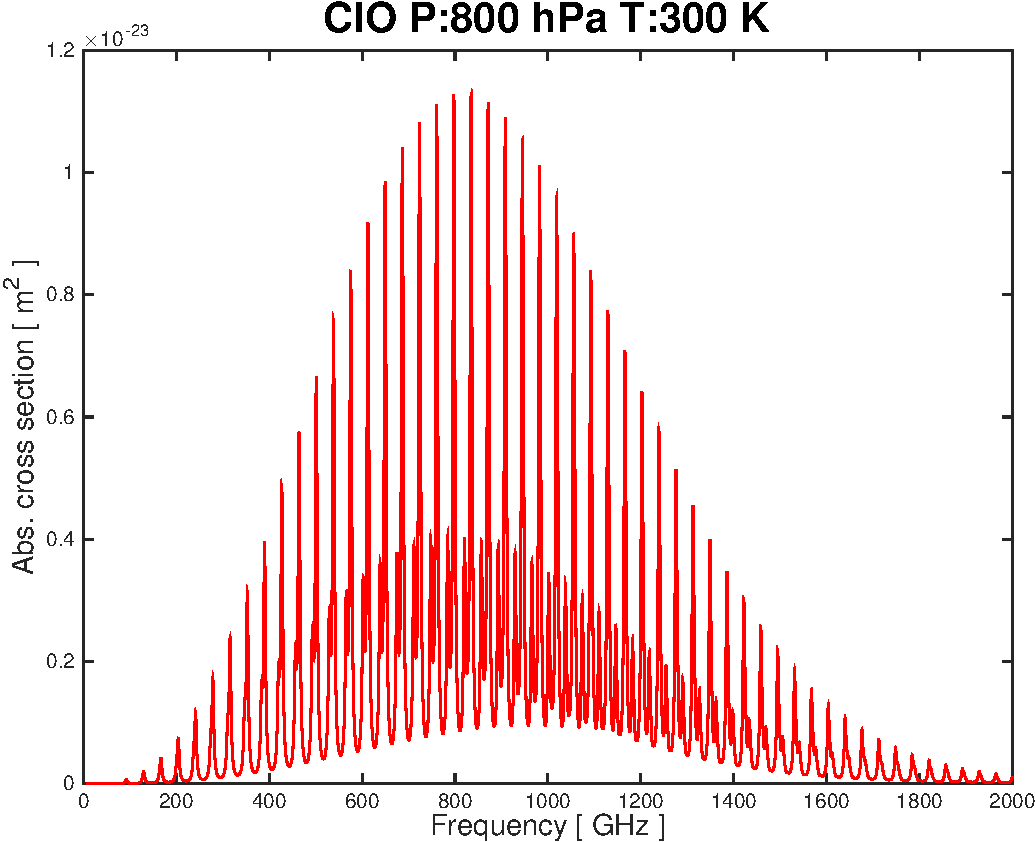
\includegraphics[width=\textwidth]{plots/plot_xsec_ClO_800hPa_300K.pdf}
 \caption{ClO}
 \end{subfigure}
 
 \caption{absorption cross sections of the molecules HCL, ClO, CO, N2O and O3.}
 \label{figure:abs_molucules}
\end{figure}

\begin{itemize}
	\item Estimate the rotational constant B for HCl and for CO. 
		\begin{itemize}
		\item 
		\end{itemize}
	\item Why is B larger for HCl than for CO?
		\begin{itemize}
		\item 
		\end{itemize}
	\item Do you have any idea why $N_{2}O$ behaves like a diatomic molecule - and $O_{3}$ not?
		\begin{itemize}
		\item 
		\end{itemize}
\end{itemize}

%----------------------------------------------------------------------------------------

\section{pressure dependency of the abs cross section}

Choose an individual line and perform calculations over a restricted frequency range for four different pressures (1hPa, 10hPa, 100hPa, 1000hPa). Keep the temperature and constituent mixing ratio constant. 

% figures abs cross sections
\begin{figure}[t!]
 \centering
 \begin{subfigure}[t]{0.45\textwidth}
 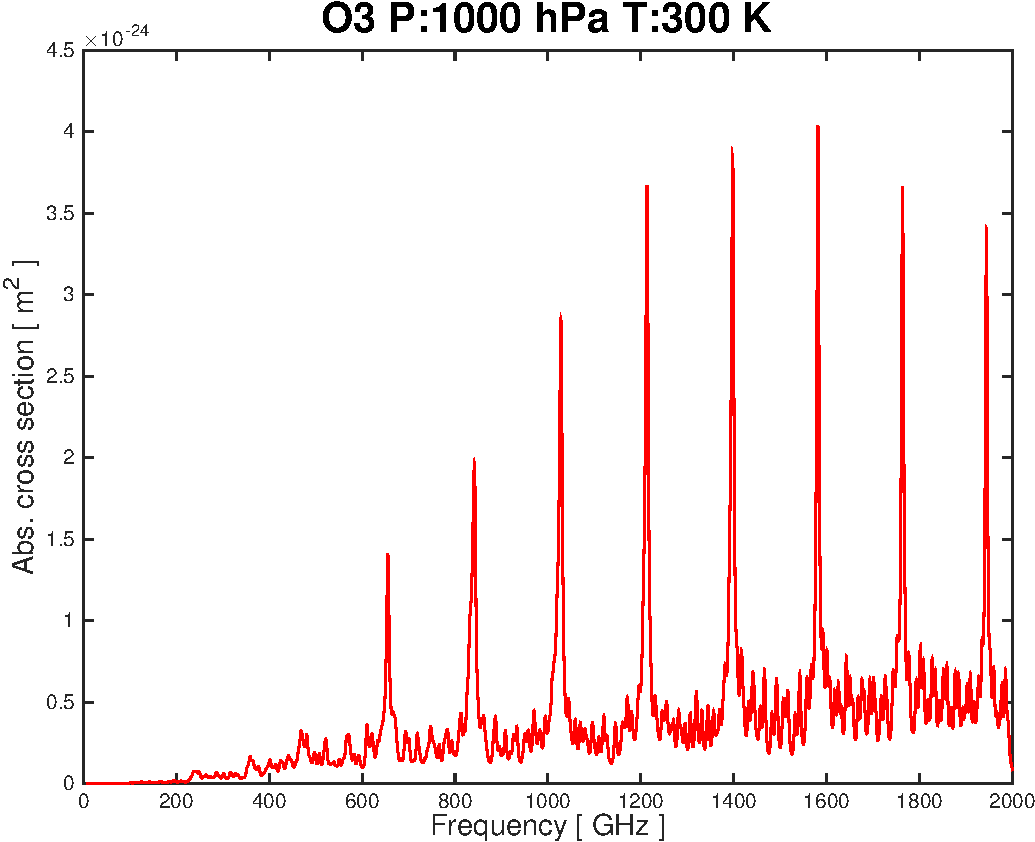
\includegraphics[width=\textwidth]{plots/plot_xsec_O3_1000hPa_300K.pdf}
 \caption{1000 hPa}
 \end{subfigure}
 \begin{subfigure}[t]{0.45\textwidth}
 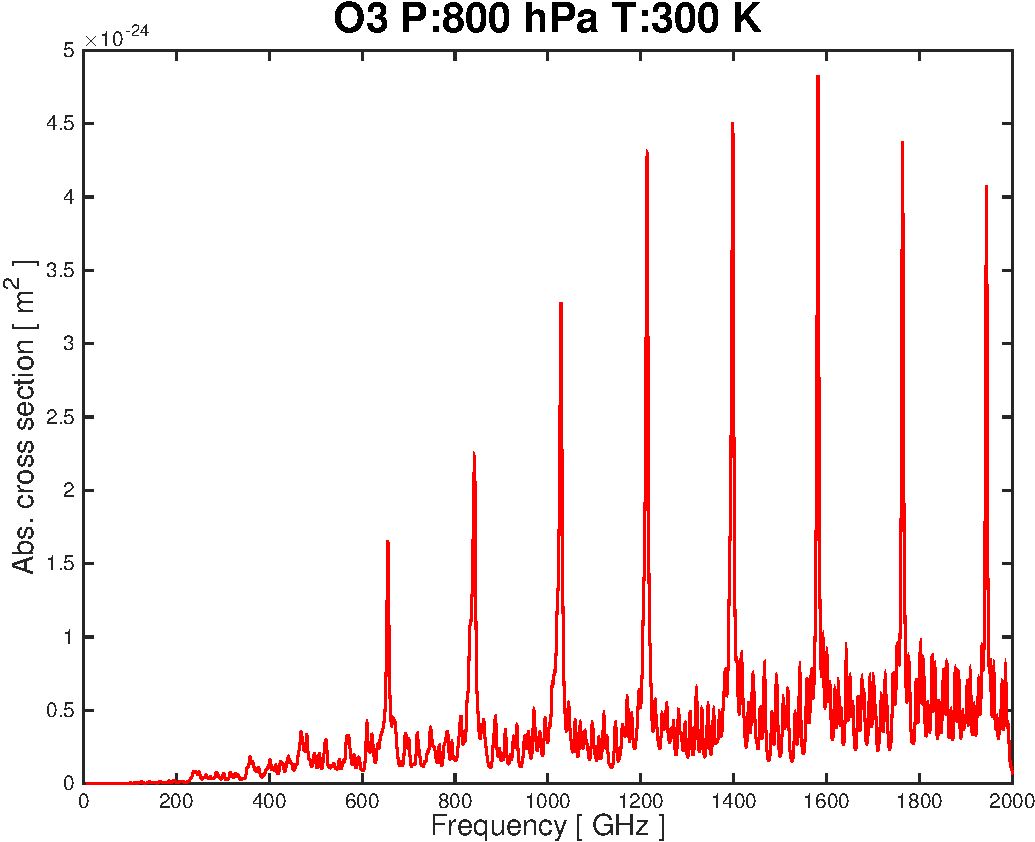
\includegraphics[width=\textwidth]{plots/plot_xsec_O3_800hPa_300K.pdf}
 \caption{800 hPa}
 \end{subfigure}
 \begin{subfigure}[b]{0.45\textwidth}
 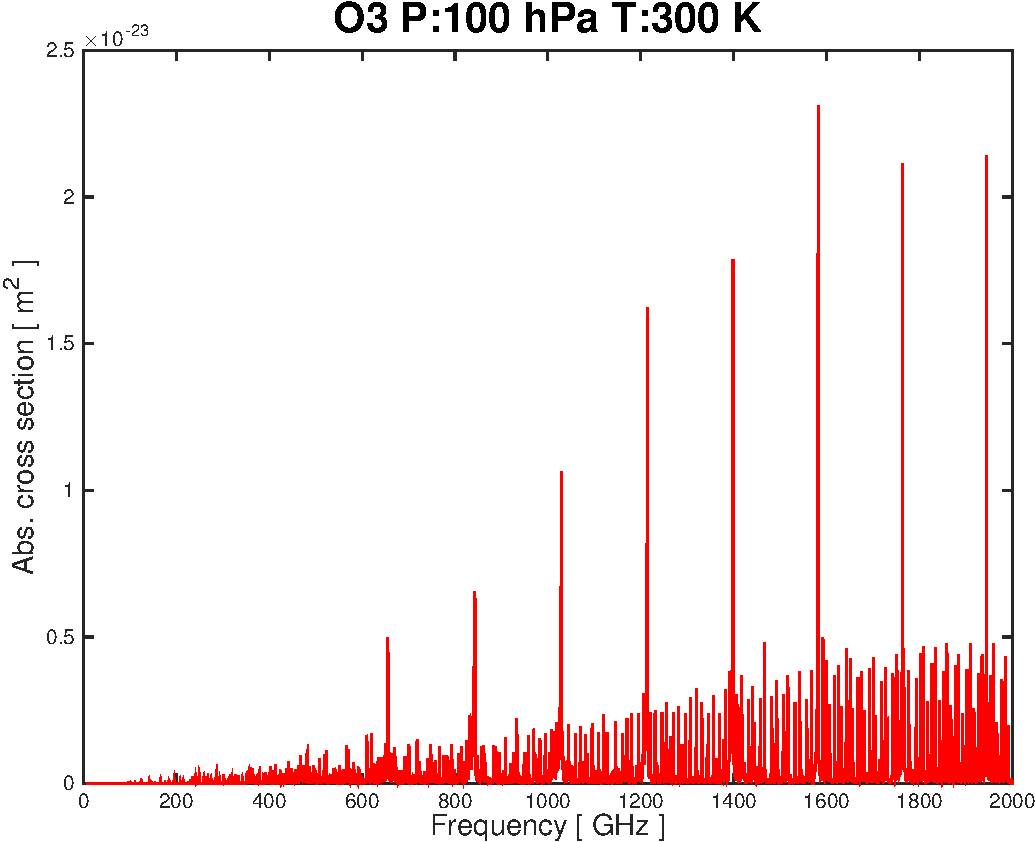
\includegraphics[width=\textwidth]{plots/plot_xsec_O3_100hPa_300K.pdf}
 \caption{100 hPa}
 \end{subfigure}
 \begin{subfigure}[b]{0.45\textwidth}
 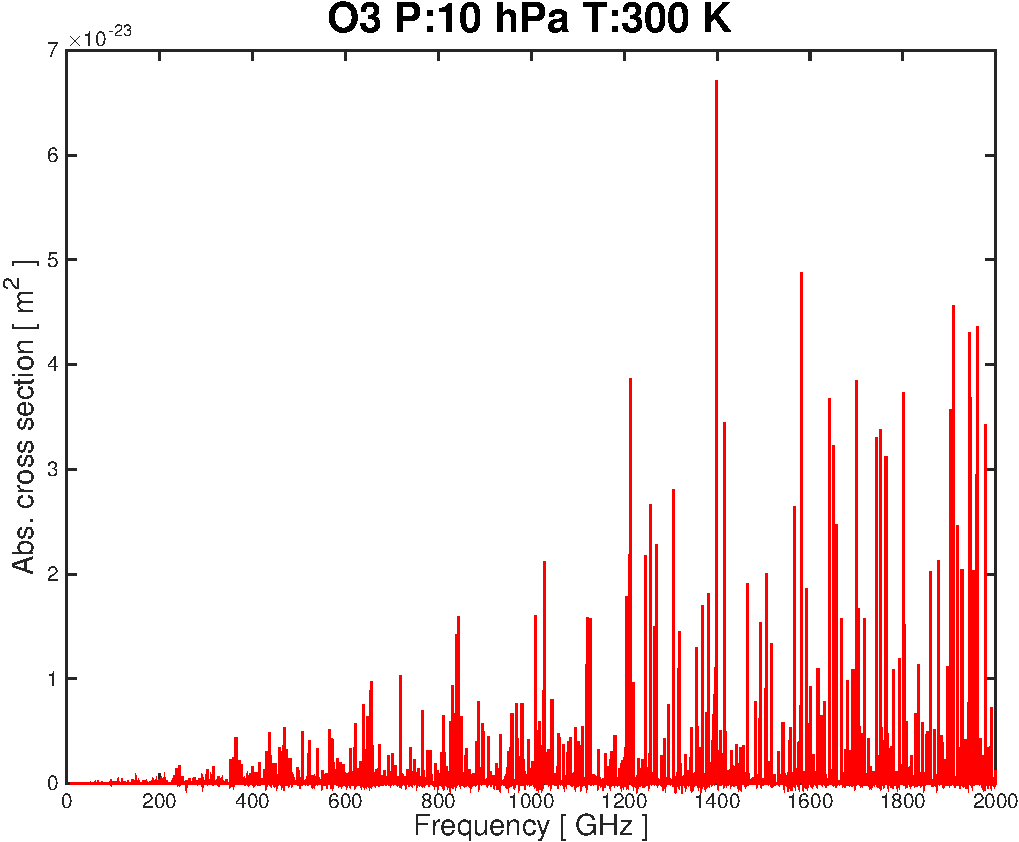
\includegraphics[width=\textwidth]{plots/plot_xsec_O3_10hPa_300K.pdf}
 \caption{10 hPa}
 \end{subfigure}
 \caption{absorption cross sections for O3 at two different pressure levels.}
 \label{figure:abs_pressure}
\end{figure}


\begin{itemize}
	\item How does the shape of the spectral lines change?
		\begin{itemize}
		\item 
		\end{itemize}
	\item How does the absoption coefficient in the line center change, if pressure is changed?
		\begin{itemize}
		\item 
		\end{itemize}
\end{itemize}

%----------------------------------------------------------------------------------------

\end{document}
